\section{Experimental Protocols and Additional Results}
\label{app:experiments}

\subsection{Common implementation contract}
All panels use frozen prompt IDs, model/checkpoint hashes, bit grids, coupling families, horizons, and event-addressed random streams. The quantizer is simulated matrix-weight, per-output-channel symmetric RTN; activations remain in the reference precision. Generated positions are scored with normalized exact-token Hamming. Complete raw tables, configs, code snapshots, and archive hashes are distributed with the supplementary artifact.

\begin{table}[ht]
\caption{Primary work packages and statistical units.}
\label{tab:app-panels}
\centering\footnotesize
\setlength{\tabcolsep}{2.5pt}
\begin{tabular}{@{}p{0.17\linewidth}p{0.12\linewidth}p{0.16\linewidth}p{0.17\linewidth}p{0.22\linewidth}@{}}
\toprule
Panel & Model & Prompt block & Simultaneous family & Top-level unit \\
\midrule
CERT-3 & MDLM 0.2B & 64 fixed, 4 draws & $K=49$, $\delta=.05$ & prompt--draw; block sensitivity \\
WP07C & MDLM 0.2B & 128 IID source prompts & $K=49$, $\delta=.05$ & prompt mean \\
WP07B & MDLM 0.2B & 64 IID source prompts & $K=91$, $\delta=.05$ & prompt mean \\
WP07D & SMDM 1.14B & 32 fixed, 2 draws & $K=50$, $\delta=.05$ & prompt--draw \\
LOCAL-LIFT & SMDM 1.14B & 32 fixed & $K=92$ or $120$ & prompt block \\
\bottomrule
\end{tabular}
\end{table}

\subsection{Fixed-suite and prompt-population certificates}
The primary fixed suite contains 64 frozen prompts at 16 generated positions. For each bit and horizon, four independently addressed CMC draws are treated as bounded prompt--draw observations in the preregistered primary analysis. A conservative sensitivity first averages the four draws within each prompt and applies concentration over 64 prompt blocks; its radius is $0.231968$, yielding full-horizon direct UCBs $0.4668/0.6363/0.9991$ at W8/W6/W4. The matched independent-FP reference at length 16 is $0.9766$; a separate 32-token intrinsic-diversity audit yields $0.9878$.

The prompt-population experiment draws 128 records IID with replacement from a frozen filtered WikiText-103 raw-train source~\citep{merity2017pointer}. The raw snapshot has $1{,}801{,}350$ rows. Unicode NFKC normalization, whitespace collapse, length and alphabetic-character filters, heading removal, and prior-prompt exclusion leave $151{,}528$ eligible records. The prompt-level simultaneous radius is $0.164026$.

\begin{table}[ht]
\caption{Absolute certified horizons for the declared prompt population. ``None'' means the simultaneous UCB exceeds the tolerance at the first nonzero horizon.}
\label{tab:app-pop-horizon}
\centering\small
\begin{tabular}{@{}llccc@{}}
\toprule
Precision & Route & $\eps=.25$ & $\eps=.50$ & $\eps=.75$\\
\midrule
W8 & $D_{\rm CMC}$ & H12 & FULL & FULL\\
W8 & $B_{\rm FS}$ & None & H12 & FULL\\
W6 & $D_{\rm CMC}$ & H8 & H24 & FULL\\
W6 & $B_{\rm FS}$ & None & H4 & H16\\
W4 & $D_{\rm CMC}$ & H4 & H12 & H24\\
W4 & $B_{\rm FS}$ & None & None & None\\
\bottomrule
\end{tabular}
\end{table}

Full-horizon trajectory-draw split probabilities are $0.5781/0.8359/1.0000$ at W8/W6/W4. Prompt-block any-split fractions are $0.8047/0.9688/1.0000$ and are reported separately. At W8, trajectory-conditional endpoint damage changes from $0.455$ on the fixed suite to $0.490$ under the source-population experiment; the panel does not support a decrease in conditional damage.

\subsection{Six-level finite-bit scaling}
The scaling study draws 64 fresh source-population prompts, split 32/32 into calibration and held-out subsets. Each prompt contributes 32 native stochastic kernels plus terminal completion. W4--W8 are used in the primary fixed-effect fit; W3 is a preregistered stress point.

\begin{table}[ht]
\caption{Six-level aggregate local and terminal quantities.}
\label{tab:app-scaling}
\centering\small
\begin{tabular}{@{}lrrrrrr@{}}
\toprule
Bit & W3 & W4 & W5 & W6 & W7 & W8\\
\midrule
One-step $W_d$ & .02366 & .01153 & .00582 & .00314 & .00185 & .00135\\
CMC split hazard & .31572 & .16739 & .08841 & .04888 & .02911 & .02133\\
Terminal $D_{\rm CMC}$ & .8662 & .7754 & .6455 & .4277 & .2695 & .2183\\
Terminal $B_{\rm FS}$ & .9722 & .9224 & .8203 & .6069 & .3794 & .3252\\
\bottomrule
\end{tabular}
\end{table}

Held-out prompt-fixed-effect slopes are $0.7855[0.7618,0.8078]$ for one-step Wasserstein cost and $0.7580[0.7346,0.7804]$ for split hazard; within-prompt $R^2$ exceeds $0.96$. Early/middle/late slopes differ, so the global exponent is a finite-range summary rather than a universal step-invariant law.

\subsection{Second model and task relevance}
The second-model panel uses the pinned 1.14B SMDM checkpoint at 16 and 64 generated positions. Its simultaneous family has $K=50$ and radius $0.232308$.

\begin{table}[ht]
\caption{SMDM full-horizon means and simultaneous one-sided UCBs.}
\label{tab:app-smdm}
\centering\small
\begin{tabular}{@{}cclrrrr@{}}
\toprule
Length & Bit & Ref. & Mean $D$ & UCB $D$ & Mean $B_{\rm FS}$ & UCB $B_{\rm FS}$\\
\midrule
16 & W8 & BF16 & .201 & .433 & .400 & .633\\
16 & W6 & BF16 & .445 & .677 & .783 & 1.000\\
16 & W4 & BF16 & .715 & .947 & .948 & 1.000\\
64 & W8 & BF16 & .367 & .599 & .669 & .901\\
64 & W6 & BF16 & .574 & .807 & .918 & 1.000\\
64 & W4 & BF16 & .761 & .993 & .990 & 1.000\\
\bottomrule
\end{tabular}
\end{table}

A separate 100-example GSM8K panel~\citep{cobbe2021gsm8k} uses the official fixed-count sampler. BF16/W8/W6/W4 exact accuracies are $51/51/50/49\%$; example-level exact McNemar $p$-values are $1.000/1.000/0.625$, with zero extraction failure. The task run is descriptive because it did not record a valid proposal coupling.

\subsection{Lifted coupling and temperature extension}
The initial lifted release contains 320 trajectories. Its $288$ length-16 trajectories contribute five horizons each and its $32$ length-64 trajectories contribute six, so $288\times5+32\times6=1{,}632$ checks. The temperature extension adds 960 paired trajectories and 4,800 checks. Across all work packages the paper records $29{,}664$ pathwise checks with zero violation; these are dependent repeated checks, not independent statistical observations.

\begin{table}[ht]
\caption{Prompt-macro terminal-cost contrast $D_{\rm CRN}-D_{\rm lift}$.}
\label{tab:app-temp-macro}
\centering\small
\begin{tabular}{@{}crrrr@{}}
\toprule
Temp. & Mean gap & 95\% bootstrap interval & Sign $p$ & Holm $p$\\
\midrule
0.0 & .00000 & $[.00000,.00000]$ & 1.000 & 1.000\\
0.5 & .00130 & $[-.00293,.00684]$ & .828 & .828\\
1.0 & .01530 & $[.00260,.03060]$ & .166 & .332\\
\bottomrule
\end{tabular}
\end{table}

\begin{table}[ht]
\caption{Conditional healing at temperature $1.0$; denominators are split trajectories.}
\label{tab:app-healing}
\centering\small
\begin{tabular}{@{}llrrrr@{}}
\toprule
Bit & Coupling & Split & Re-agree & $P(\text{re-agree}\mid\text{split})$ & $P(\text{terminal eq.}\mid\text{split})$\\
\midrule
W8 & Lifted & 13 & 12 & .923 & .923\\
W8 & CRN & 19 & 15 & .789 & .789\\
W6 & Lifted & 28 & 23 & .821 & .821\\
W6 & CRN & 26 & 25 & .962 & .923\\
W4 & Lifted & 52 & 44 & .846 & .731\\
W4 & CRN & 57 & 47 & .825 & .684\\
\bottomrule
\end{tabular}
\end{table}

\begin{figure}[ht]
\centering
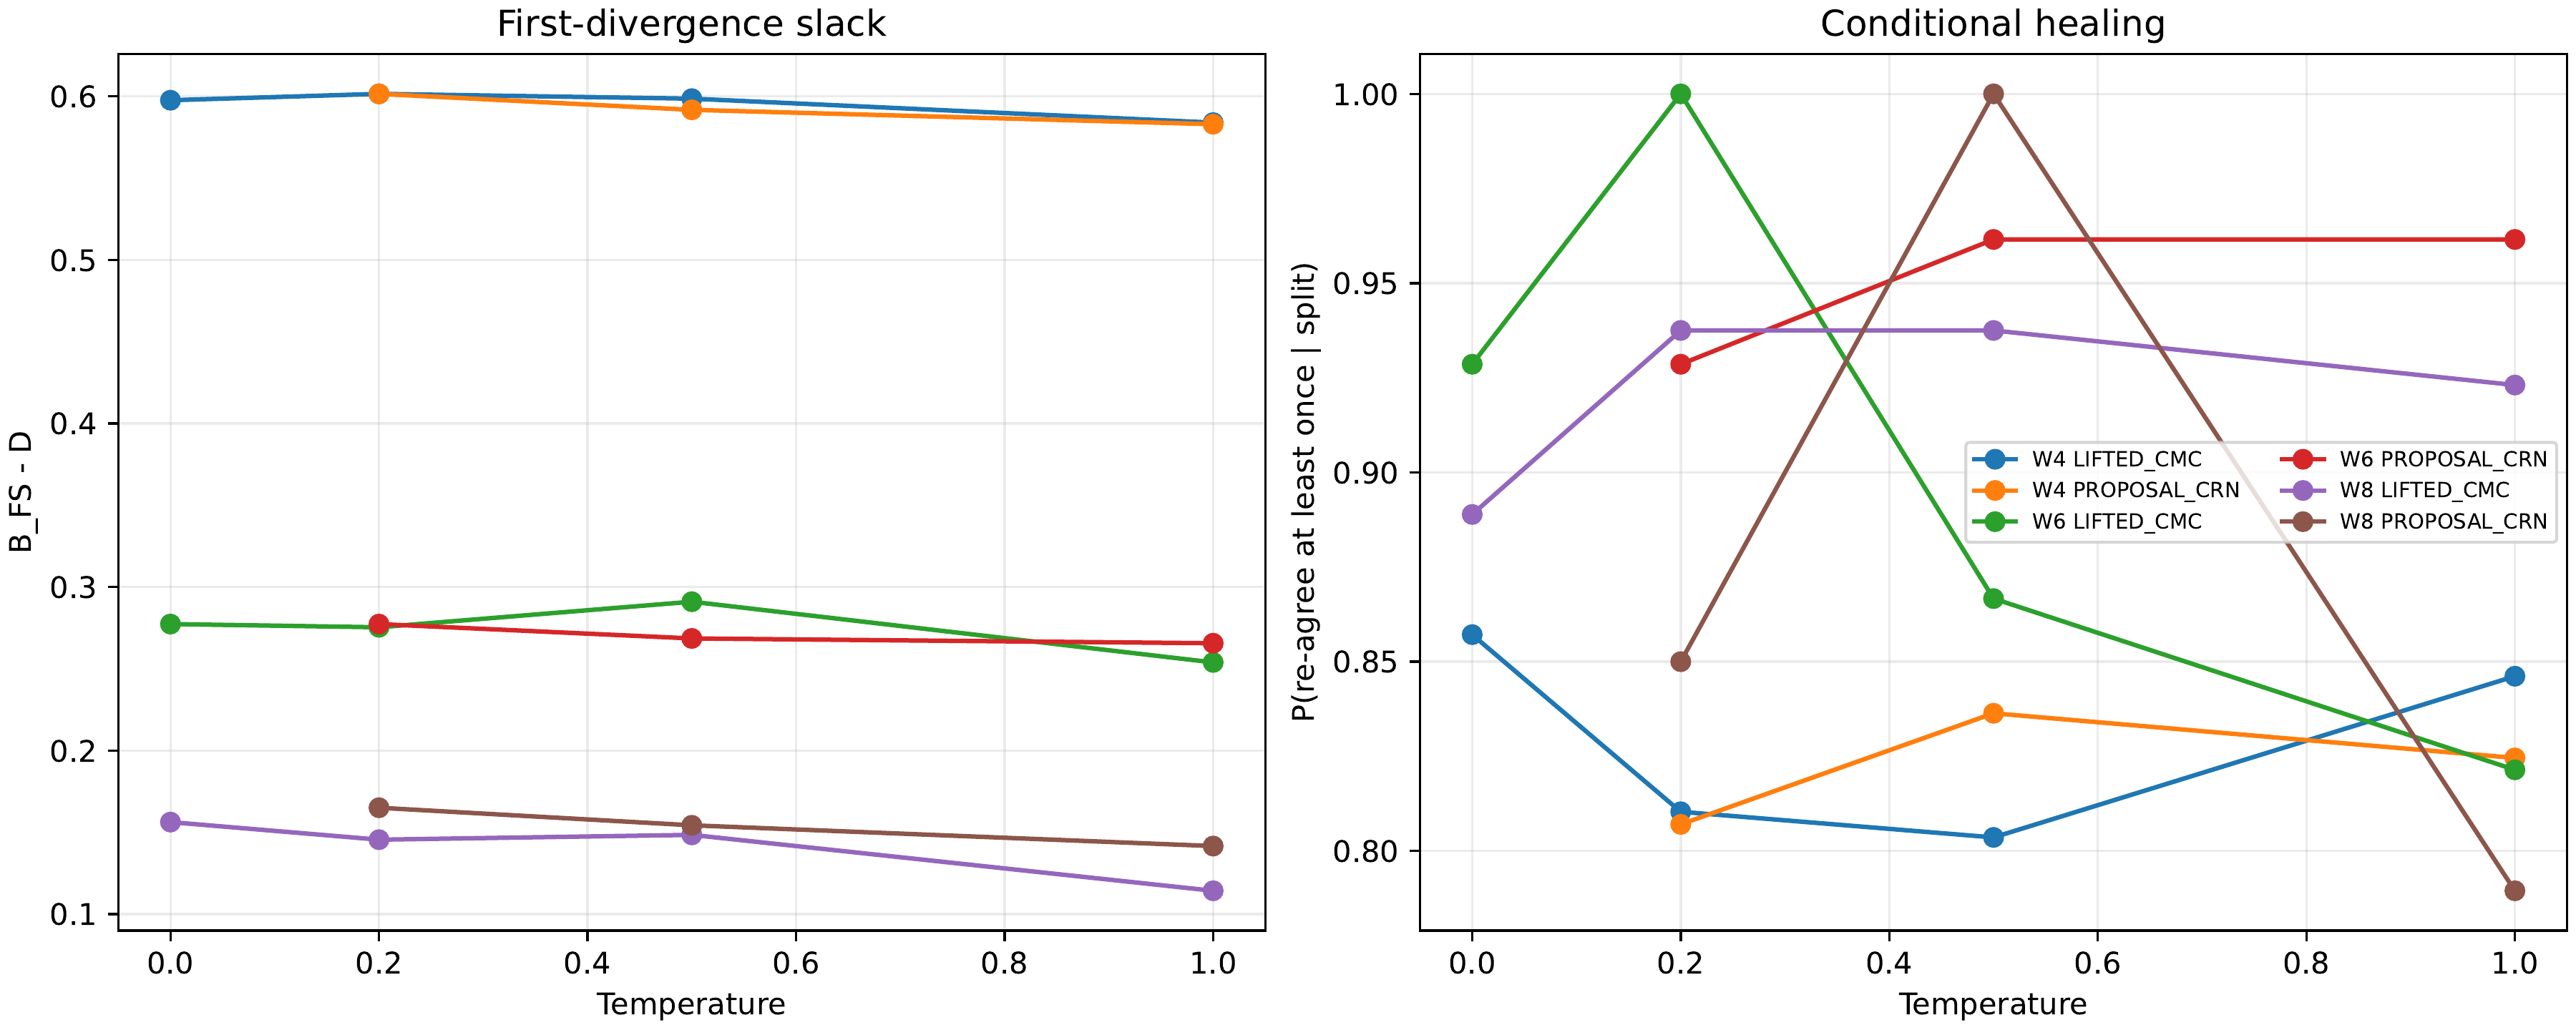
\includegraphics[width=.83\linewidth]{figures/figure_temperature_healing.png}
\caption{First-divergence slack and exact conditional healing. Healing is conditioned on a first split and exhibits the same mixed, bit-dependent ordering as terminal cost.}
\label{fig:app-healing}
\end{figure}

The same-state audit spans early/middle/late states, both precision branches, and 4,000 draws per route. At temperature $1.0$, mean proposal effective support is $1.934$, mean pushed-forward support $1.074$, maximum pushed-forward support $1.449$, and minimum modal probability $0.8173$. Lifted proposal-CMC reduces proposal-vector mismatch from $0.1709$ to $0.0724$, but next-state mismatch remains $0.0146$ versus $0.0142$, demonstrating selector compression.

\subsection{Negative results and interpretation limits}
All relative-to-reference-diversity certificates fail at the preregistered thresholds. First-divergence bounds can be loose because they ignore healing. The temperature comparison is mixed across bit and prompt. Exact-token Hamming is the theorem-aligned metric, not a semantic-quality certificate. The dedicated alternate-metric, lower-bound, and calibration investigations are reported in Appendix~\ref{app:negative}.
